% ============================================================
%  Semana 11 · Clase 21: Storytelling con datos: del hallazgo a la decisión
%  Curso: Análisis y Visualización de Datos para la Toma de Decisiones
%
%  Formato de la sesión (3 h):
%    Hora 1. Audiencia, mensaje principal y estructura de la narrativa
%            (contexto, tensión, evidencia, recomendación)
%    Hora 2. Diapositivas que se entienden: jerarquía visual, carga
%            cognitiva y uso responsable de los datos
%    Hora 3. Actividad en parejas o individual: una historia de 5 a 7
%            diapositivas para una audiencia directiva
%
%  Caso: Cafés Altavista (Clase 16, datos/cafes_altavista.xlsx de esa
%  clase). Figuras: figuras/*.pdf, con ../../../scripts/semana11-clase21_figuras.py.
%
%  Compilar (dos veces) directamente desde esta carpeta:
%    xelatex semana11-clase21.tex
%    xelatex semana11-clase21.tex
% ============================================================
\documentclass[aspectratio=169,11pt]{beamer}

\usepackage{../../../plantilla/beamerthemeesumer}
\usetheme{esumer}

\usepackage[spanish,es-noshorthands]{babel}
\usepackage{booktabs}
\usepackage{graphicx}
\usepackage{array}
\newcolumntype{L}[1]{>{\raggedright\arraybackslash}p{#1}}
\usetikzlibrary{arrows.meta,positioning,calc}
\tikzset{every node/.append style={execute at begin node={\hyphenpenalty=10000\exhyphenpenalty=10000\relax}}}

% ---------------- DATOS DE LA CLASE ----------------
\title{Storytelling con datos}
\subtitle{Del hallazgo a la decisión}
\author{Docente: Cristian A. Jimenez C., MSc}
\date{Nov 17 al 22}

\setmodulo{Módulo 4: Innovar (Analítica Predictiva y Storytelling)}
\setsemana{11}
\setclase{21}
\setfechaclase{Nov 17 al 22}
\setmodalidad{Virtual}
% -----------------------------------------------------

\graphicspath{{figuras/}}

\newcommand{\fuentedatos}{\par\vspace{1pt}{\fontsize{5.5}{6.5}\selectfont\color{black!55}%
  Datos simulados de Cafés Altavista S.A.S., empresa ficticia del curso (Clase 16).\par}}

\begin{document}

{
\setbeamertemplate{footline}{}
\begin{frame}[plain,noframenumbering]
  \titlepage
\end{frame}
}

\begin{frame}[t]{Agenda de hoy (3 horas)}
  \begin{columns}[T,onlytextwidth]
    \column{0.32\textwidth}
    \begin{block}{Hora 1}
      \small Audiencia, mensaje en una frase y estructura: contexto,
      tensión, evidencia y recomendación.
    \end{block}
    \column{0.32\textwidth}
    \begin{block}{Hora 2}
      \small Diapositivas que se entienden: jerarquía visual, carga
      cognitiva y uso responsable de los datos.
    \end{block}
    \column{0.32\textwidth}
    \begin{block}{Hora 3}
      \small Actividad, en parejas o individual: tu historia en 5 a 7
      diapositivas.
    \end{block}
  \end{columns}
  \vspace{0.3cm}
  \small Ya sabes encontrar hallazgos (Módulo 3) y predecir (Clases 19 y
  20). Pero un hallazgo que nadie entiende no cambia ninguna decisión. Hoy
  aprendes a contarlo.
\end{frame}

\begin{frame}[t]{Del tablero a la historia}
  \begin{columns}[T,onlytextwidth]
    \column{0.48\textwidth}
    \begin{block}{Un tablero (Clases 14 y 15)}
      \small
      \begin{itemize}
        \small
        \item Sirve para \textbf{explorar}.
        \item Responde muchas preguntas.
        \item Quien lo usa elige qué mirar y filtra.
      \end{itemize}
    \end{block}
    \column{0.48\textwidth}
    \begin{exampleblock}{Una historia (hoy)}
      \small
      \begin{itemize}
        \small
        \item Sirve para \textbf{decidir}.
        \item Responde una pregunta, con una recomendación.
        \item Tú guías: cada diapositiva lleva a la siguiente.
      \end{itemize}
    \end{exampleblock}
  \end{columns}
  \vspace{0.3cm}
  \small El error más común: llevar el tablero al comité y recorrerlo
  gráfico por gráfico. La gerencia no quiere ver todo lo que encontraste:
  quiere saber \textbf{qué hacer}.
\end{frame}

% ============================================================
\section{Hora 1: Audiencia, mensaje y estructura}
% ============================================================
\begin{frame}[t]{Primero, la audiencia}
  \small Antes de abrir Canva o Google Slides, responde cuatro preguntas:
  \vspace{0.1cm}

  \footnotesize
  \renewcommand{\arraystretch}{1.3}
  \begin{tabular}{@{}L{3.4cm}L{10.1cm}@{}}
    \toprule
    \textbf{Pregunta} & \textbf{En el caso de Cafés Altavista} \\
    \midrule
    ¿Quién decide? & La gerencia general, en el comité de octubre. \\
    ¿Qué le importa? & Vender más, sin perder margen: la meta es un margen de al menos el 60\%. \\
    ¿Cuánto tiempo tiene? & Cinco minutos para este tema. \\
    ¿Qué sabe ya? & Conoce el negocio y la campaña de septiembre. No conoce Power BI ni sabe qué es una regresión. \\
    \bottomrule
  \end{tabular}
  \vspace{0.2cm}
  \begin{alertblock}{La regla}
    \footnotesize Habla en el idioma de quien decide: pesos, metas y
    clientes. No ``la medida DAX'', ``el coeficiente'' ni ``el $R^2$''.
  \end{alertblock}
\end{frame}

\begin{frame}[t]{El mensaje, en una frase}
  \small Si la audiencia solo recordara una frase, ¿cuál sería? Escríbela
  antes de hacer cualquier diapositiva.
  \vspace{0.15cm}
  \begin{center}
  \begin{tikzpicture}[
    pz/.style={draw=none, rounded corners=3pt, text=white, align=center, font=\footnotesize,
               minimum height=1.1cm, text width=3.5cm, inner sep=4pt},
  ]
    \node[pz, fill=esumerSky] at (2.1,0) {\textbf{Qué pasó}};
    \node[pz, fill=esumerOrange] at (6.6,0) {\textbf{Por qué importa}};
    \node[pz, fill=esumerTeal] at (11.1,0) {\textbf{Qué proponemos}};
    \node at (4.35,0) {\Large +};
    \node at (8.85,0) {\Large +};
  \end{tikzpicture}
  \end{center}
  \begin{exampleblock}{Ejemplo con Cafés Altavista}
    \small ``Septiembre fue récord de ventas gracias a la campaña del café
    en grano, pero el margen cayó por debajo de la meta: proponemos
    repetirla con menos descuento.''
  \end{exampleblock}
  \footnotesize Si tu frase no cabe en dos líneas, o no dice qué hacer,
  todavía no tienes claro el mensaje. La recomendación del ejemplo es una
  propuesta para la clase; la decide la empresa.
\end{frame}

\begin{frame}[t]{La estructura de la historia}
  \begin{center}
  \begin{tikzpicture}[
    tit/.style={draw=none, rounded corners=3pt, text=white, font=\small\bfseries,
                minimum width=3.1cm, minimum height=0.7cm},
    txt/.style={draw=esumerNavy!40, rounded corners=2pt, fill=white, align=left,
                text width=2.9cm, font=\scriptsize, inner sep=4pt, anchor=north,
                minimum height=2.9cm},
    fl/.style={-{Stealth[length=2.2mm]}, line width=0.9pt, color=esumerNavy},
  ]
    \node[tit, fill=esumerSky] (a) at (1.6,0) {Contexto};
    \node[tit, fill=esumerOrange] (b) at (5.2,0) {Tensión};
    \node[tit, fill=esumerNavy] (c) at (8.8,0) {Evidencia};
    \node[tit, fill=esumerTeal] (d) at (12.4,0) {Recomendación};
    \draw[fl] (a) -- (b); \draw[fl] (b) -- (c); \draw[fl] (c) -- (d);
    \node[txt] at (1.6,-0.5) {\textbf{Dónde estamos.}\\[2pt]Septiembre fue el mejor mes del año: 89,2 millones en ventas, 20,5\% más que agosto.};
    \node[txt] at (5.2,-0.5) {\textbf{El problema.}\\[2pt]Pero el margen cayó a 56,6\%, por debajo de la meta del 60\%. Once meses estuvo entre 63\% y 64\%.};
    \node[txt] at (8.8,-0.5) {\textbf{Por qué pasó.}\\[2pt]El 25\% de descuento en café en grano triplicó sus unidades (de 281 a 900) y bajó su margen de 54,1\% a 39,5\%.};
    \node[txt] at (12.4,-0.5) {\textbf{Qué hacer.}\\[2pt]Repetir la campaña con menos descuento, o solo para socios, y medir el margen además de las ventas.};
  \end{tikzpicture}
  \end{center}
  \vspace{-0.1cm}
  \footnotesize La \textbf{tensión} es lo que hace que la audiencia
  escuche: sin un problema, no hay nada que decidir.
  \fuentedatos
\end{frame}

\begin{frame}[t]{Del guion a las diapositivas}
  \small Cada parte de la estructura es una o dos diapositivas, y cada una
  tiene un \textbf{título que concluye}:
  \vspace{0.15cm}
  \begin{center}
  \begin{tikzpicture}[
    sl/.style={draw=esumerNavy!60, line width=0.6pt, rounded corners=2pt, fill=white,
               minimum width=2.45cm, minimum height=1.6cm, text width=2.25cm, align=left,
               font=\scriptsize, inner sep=3pt},
    num/.style={circle, fill=esumerOrange, text=white, font=\tiny\bfseries,
                inner sep=0pt, minimum size=0.38cm},
    et/.style={font=\scriptsize\bfseries, text=esumerNavy},
  ]
    \foreach \x/\t/\e [count=\i] in {
      1.3/{Septiembre: récord de ventas del año}/Contexto,
      4.08/{Pero el margen cayó por debajo de la meta}/Tensión,
      6.86/{La causa: el 25\% de descuento en café en grano}/Evidencia,
      9.64/{Aun así, el margen en pesos subió 3,6 millones}/Evidencia,
      12.42/{Propuesta: repetir la campaña con menos descuento}/Recomendación} {
      \node[sl] (s\i) at (\x,0) {\t};
      \node[num] at (s\i.north west) {\i};
      \node[et] at (\x,-1.15) {\e};
    }
  \end{tikzpicture}
  \end{center}
  \begin{columns}[T,onlytextwidth]
    \column{0.48\textwidth}
    \begin{block}{La diapositiva 4 es honestidad}
      \footnotesize El margen en pesos sí subió (de 46,8 a 50,5 millones).
      Decirlo hace creíble el resto. Esconderlo, si alguien lo descubre,
      tumba toda la presentación.
    \end{block}
    \column{0.48\textwidth}
    \begin{block}{Prueba del guion}
      \footnotesize Lee solo los títulos, en orden. Si cuentan la historia
      completa, el guion funciona.
    \end{block}
  \end{columns}
  \fuentedatos
\end{frame}

\begin{frame}[t]{Títulos que concluyen}
  \small El título dice la \textbf{conclusión}, no el tema (Clase 11):
  \vspace{0.1cm}

  \footnotesize
  \renewcommand{\arraystretch}{1.35}
  \begin{tabular}{@{}L{5.2cm}L{8.3cm}@{}}
    \toprule
    \textbf{Así no} & \textbf{Así sí} \\
    \midrule
    Ventas por mes & Septiembre: récord de ventas del año, 89,2 millones \\
    Margen \% mensual & Por primera vez en el año, el margen quedó bajo la meta del 60\% \\
    Unidades por categoría & El café en grano triplicó sus unidades con el 25\% de descuento \\
    Resultados del modelo & Con el clima y el calendario, el error diario baja a la mitad (Clase 20) \\
    \bottomrule
  \end{tabular}
  \vspace{0.2cm}
  \begin{alertblock}{Ojo}
    \footnotesize En un tablero con segmentadores el título dice la
    \emph{pregunta}, porque las cifras cambian al filtrar (Clase 15). En una
    presentación las cifras están fijas: ahí sí, el título concluye.
  \end{alertblock}
  \fuentedatos
\end{frame}

% ============================================================
\section{Hora 2: Diapositivas que se entienden}
% ============================================================
\begin{frame}[t]{Jerarquía visual: el mismo dato, dos veces}
  \begin{columns}[T,onlytextwidth]
    \column{0.49\textwidth}
    \centering
    {\small\bfseries\color{esumerOrange} Antes}\\[2pt]
    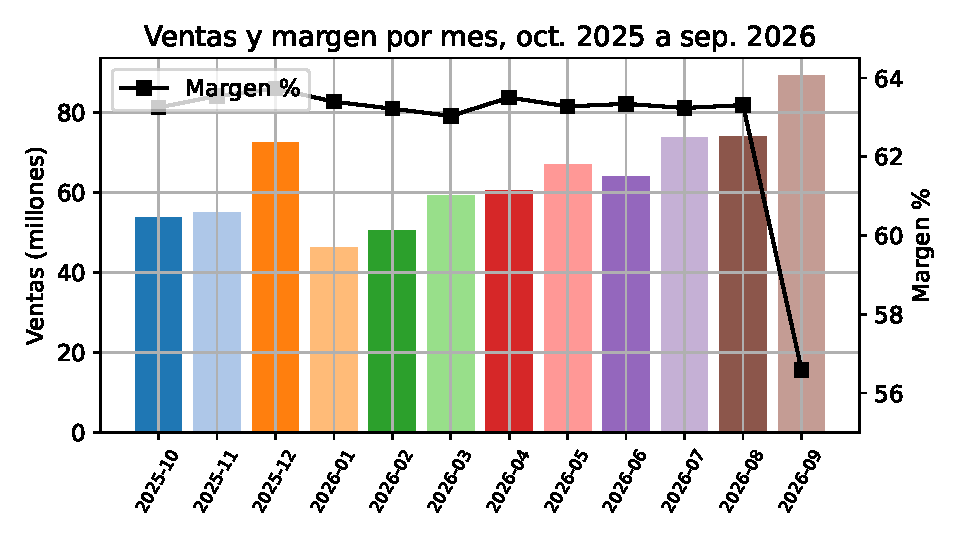
\includegraphics[width=\linewidth,height=4.1cm,keepaspectratio]{fig_antes.pdf}\\[2pt]
    \raggedright\scriptsize Doble eje, un color por mes que no significa
    nada, rejilla, leyenda y un título que solo describe. ¿Dónde mirar?
    \column{0.49\textwidth}
    \centering
    {\small\bfseries\color{esumerTeal} Después}\\[2pt]
    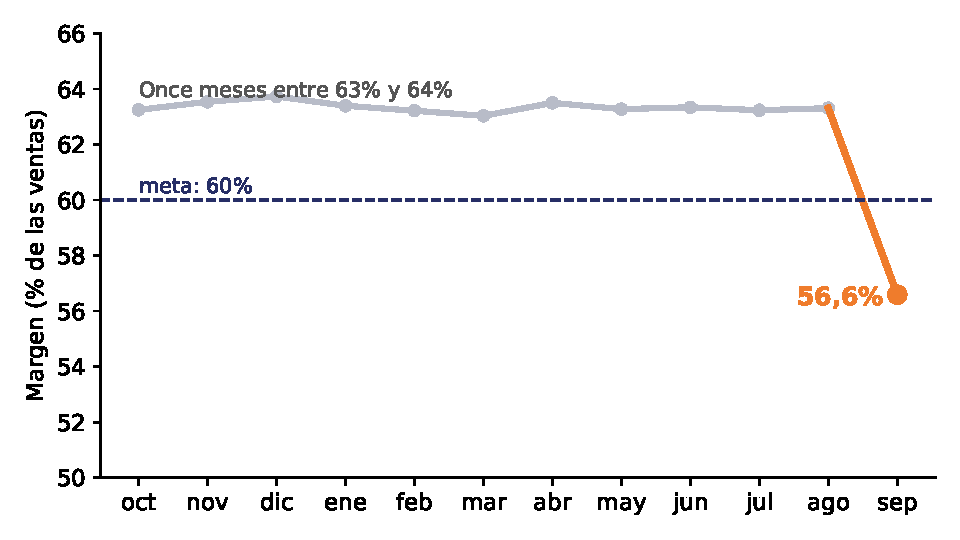
\includegraphics[width=\linewidth,height=4.1cm,keepaspectratio]{fig_despues.pdf}\\[2pt]
    \raggedright\scriptsize Una sola pregunta (el margen), gris para el
    contexto, naranja para el mensaje y la meta como referencia. El ojo va
    directo a septiembre.
  \end{columns}
  \vspace{0.1cm}
  \footnotesize\textbf{Título para la diapositiva de la derecha:} ``Por
  primera vez en el año, el margen quedó bajo la meta del 60\%''.
  \fuentedatos
\end{frame}

\begin{frame}[t]{Cómo bajar la carga cognitiva}
  \small La audiencia tiene atención limitada: cada elemento que no aporta
  le quita atención al mensaje.
  \vspace{0.1cm}
  \begin{columns}[T,onlytextwidth]
    \column{0.5\textwidth}
    \begin{enumerate}
      \footnotesize
      \item \textbf{Una idea por diapositiva.} Si hay dos, son dos
        diapositivas.
      \item \textbf{Gris para el contexto, un color para el mensaje.}
      \item \textbf{Texto sobre el gráfico}, junto al dato, en vez de
        leyendas.
      \item \textbf{Quita lo que sobra}: rejillas, bordes, decimales,
        logos repetidos.
    \end{enumerate}
    \column{0.46\textwidth}
    \begin{enumerate}
      \footnotesize
      \setcounter{enumi}{4}
      \item \textbf{Cifras redondas al hablar}: ``89 millones'', no
        ``89.161.940''.
      \item \textbf{Un orden de lectura claro}: título, gráfico y una nota
        corta.
      \item \textbf{Poco texto}: lo que dirías en voz alta no va escrito en
        la diapositiva.
    \end{enumerate}
  \end{columns}
  \vspace{0.15cm}
  \begin{block}{Prueba de los cinco segundos}
    \footnotesize Muestra la diapositiva cinco segundos y quítala. Si
    alguien no puede decir cuál era el mensaje, sobra algo.
  \end{block}
\end{frame}

\begin{frame}[t]{Uso responsable de los datos}
  \small Una historia convincente también puede engañar. Antes de
  presentar, revisa:
  \vspace{0.1cm}

  \footnotesize
  \renewcommand{\arraystretch}{1.25}
  \begin{tabular}{@{}L{3.6cm}L{9.9cm}@{}}
    \toprule
    \textbf{Riesgo} & \textbf{Qué hacer} \\
    \midrule
    Escalas que exageran & Barras desde cero; sin doble eje (Clase 11). \\
    Elegir el periodo que conviene & Compara periodos equivalentes y dilo en el título. \\
    Callar lo que no conviene & Si el margen en pesos subió, dilo, aunque tu mensaje sea que el margen \% bajó. \\
    Vender relación como causa & ``Se asocia con'', no ``causa'', salvo con un experimento (Clase 19). \\
    Predecir sin el error & Una predicción va con su error: ``unas 6371 bicicletas, con un error típico de unas 730'' (Clase 20). \\
    Exponer personas & Nada de nombres, correos ni datos de socios en las diapositivas (Clase 1). \\
    \bottomrule
  \end{tabular}
\end{frame}

% ============================================================
\section{Actividad}
% ============================================================
\begin{frame}[t]{Actividad: tu historia en 5 a 7 diapositivas}
  \begin{columns}[T,onlytextwidth]
    \column{0.55\textwidth}
    \small En \textbf{parejas} o \textbf{individual}:
    \begin{enumerate}
      \footnotesize
      \item \textbf{Elige el caso}: tu proyecto, o uno del curso
        (gimnasio, Cafés Altavista o bicicletas).
      \item \textbf{Ficha de audiencia}: las cuatro preguntas.
      \item \textbf{El mensaje en una frase}: qué pasó, por qué importa y
        qué proponen.
      \item \textbf{El guion}: de 5 a 7 diapositivas, con contexto,
        tensión, evidencia y recomendación. Primero solo los títulos.
      \item \textbf{Un gráfico rediseñado}: toma uno de tu tablero y
        aplícale la jerarquía visual.
      \item \textbf{Ensayo}: cuenten la historia en tres minutos.
    \end{enumerate}
    \column{0.41\textwidth}
    \begin{block}{En parejas}
      \footnotesize Uno cuenta y el otro hace de gerente: interrumpe con
      ``¿y eso qué significa para mí?''. Al final, el que escuchó revisa la
      lista de chequeo. Luego cambian.
    \end{block}
    \begin{block}{Individual}
      \footnotesize Grábate tres minutos con el celular, mírate y revisa la
      lista de chequeo como si fueras la gerencia.
    \end{block}
    \footnotesize Herramienta: Canva o Google Slides.
  \end{columns}
\end{frame}

\begin{frame}[t]{Lista de chequeo y producto esperado}
  \begin{columns}[T,onlytextwidth]
    \column{0.55\textwidth}
    \small\textbf{Tu historia está lista cuando\ldots}
    \vspace{0.05cm}
    \begin{itemize}
      \footnotesize
      \item[$\square$] La frase del mensaje cabe en dos líneas y dice qué
        hacer.
      \item[$\square$] Hay una tensión clara: un problema o una
        oportunidad.
      \item[$\square$] Leídos en orden, los títulos cuentan la historia.
      \item[$\square$] Cada diapositiva tiene una sola idea.
      \item[$\square$] El color señala el mensaje, no decora.
      \item[$\square$] No hay escalas engañosas ni datos personales.
      \item[$\square$] La recomendación dice qué, quién y cuándo.
      \item[$\square$] Se cuenta en tres minutos.
    \end{itemize}
    \column{0.41\textwidth}
    \begin{exampleblock}{Producto}
      \footnotesize
      \begin{enumerate}
        \footnotesize
        \item La ficha de audiencia y la frase del mensaje.
        \item El guion de 5 a 7 diapositivas (Canva o Google Slides),
          con títulos que concluyen.
        \item El gráfico rediseñado, antes y después.
      \end{enumerate}
    \end{exampleblock}
    \footnotesize En la Clase 23 presentarás una versión mejorada de esta
    historia.
  \end{columns}
\end{frame}

% ============================================================
\section{Cierre}
% ============================================================
\begin{frame}[t]{Cierre y próxima sesión}
  \begin{itemize}
    \small
    \item Primero la audiencia: quién decide, qué le importa y cuánto tiempo
      tiene.
    \item El mensaje en una frase: qué pasó, por qué importa y qué proponer.
    \item Contexto, tensión, evidencia y recomendación; títulos que
      concluyen.
    \item Gris para el contexto, un color para el mensaje, una idea por
      diapositiva.
    \item Una buena historia no esconde lo que no conviene.
  \end{itemize}
  \vspace{0.15cm}
  \begin{block}{Próxima sesión: Clase 22}
    \small El argumento ejecutivo y las métricas de impacto: ¿funcionó la
    campaña de septiembre? Depende de lo que midas.
  \end{block}
\end{frame}

\begin{frame}[t]{Para seguir aprendiendo}
  \small
  \begin{block}{\emph{Storytelling with Data}, de Cole Nussbaumer Knaflic}
    \footnotesize El libro de referencia sobre el tema (Wiley, 2015). En
    español: \emph{Storytelling con datos: visualización de datos para
    profesionales} (Anaya Multimedia, 2017), y su cuaderno de ejercicios,
    \emph{Storytelling con datos: ejemplos prácticos} (Anaya, 2021).
    Pregunta por ellos en la biblioteca.
    \begin{itemize}
      \footnotesize
      \item \href{https://www.storytellingwithdata.com/book}{\color{esumerOrange}Muestra gratuita oficial}:
        la introducción y los capítulos 1 y 17.
      \item \href{https://www.storytellingwithdata.com/blog}{\color{esumerOrange}Blog de la autora}:
        ejemplos de antes y después, gratis.
    \end{itemize}
  \end{block}
  \begin{exampleblock}{Libre y completo en línea}
    \footnotesize Claus O. Wilke, \emph{Fundamentals of Data Visualization}
    (O'Reilly, 2019), con licencia Creative Commons. Para hoy, el
    \href{https://clauswilke.com/dataviz/telling-a-story.html}{\color{esumerOrange}capítulo 29: contar una historia y defender una idea}.
    \href{https://clauswilke.com/dataviz/}{\color{esumerOrange}Libro completo}.
  \end{exampleblock}
  \scriptsize Los dos libros están en inglés, salvo la edición de Anaya.
\end{frame}

{
\setbeamertemplate{footline}{}
\begin{frame}[plain,noframenumbering]
  \begin{tikzpicture}[remember picture,overlay]
    \fill[esumerNavy] (current page.south west) rectangle (current page.north east);
    \node at (current page.center) {\color{white}\Huge\bfseries ¡Gracias!};
  \end{tikzpicture}
\end{frame}
}

\end{document}
